\documentclass[10pt]{article}

\usepackage{spheric}
%%%TITLE
\title{A comparative study of SPH and MPM in modeling mixed-mode failure in rocks}
\date{}

%%AFFILIATIONS
\author[$\relax$]{Sam Raymond$^\dagger$}
\author[$\relax$]{Bruce Jones}
\author[$\relax$]{John Williams}
\affil[$\relax$]{Geonumerics Group, Department of Civil and Environmental Engineering, MIT, USA}
\affil[$\relax$]{\email{\dagger}{sjr@mit.edu}}


%%DOCUMENT
\begin{document}

\maketitle

%\SelectedTopics{}

%%PLEASE PUT YOUR ABSTRACT HERE
\begin{abstract}
In this work coupled Drucker-Prager plasticity and Grady-Kipp damage models are used to simulate mode I and mode II failure in rocks, with differing computational approaches. A previous study found that this combination of constitutive models, and the smoothed particle hydrodynamics (SPH) method, compares well with experimental results \cite{douillet2016mixed}. Here we compare this previous approach to a new framework which takes advantage of the Material Point Method (MPM) instead. MPM is a hybrid grid-particle method, which shares many similarities with SPH and has been gaining in popularity. However, as a numerical method it is still in development and much of its abilities have yet to be fully examined. SPH, being a much more developed and more widely adopted technique, is an ideal candidate for comparison. A series of different configurations of flaws within a rock specimen are modeled using the two methods with the same coupled plasticity and damage framework. These specimens are compressed to failure and the failure paths, both tensile and shear, are tracked. The two methods are compared against experimental results and the implications are discussed.


\begin{figure}[!htb]
\centering
\fbox{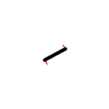
\includegraphics[width=0.25\textwidth]{4-11.png}}\hspace{1em}
\fbox{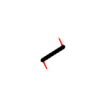
\includegraphics[width=0.25\textwidth]{4-12.png}}\hspace{1em}
\fbox{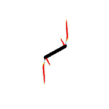
\includegraphics[width=0.25\textwidth]{4-13.png}}

\vspace{1em}

\fbox{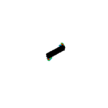
\includegraphics[width=0.25\textwidth]{4-14.png}}\hspace{1em}
\fbox{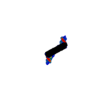
\includegraphics[width=0.25\textwidth]{4-15.png}}\hspace{1em}
\fbox{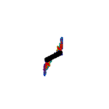
\includegraphics[width=0.25\textwidth]{4-16.png}}
\caption{A single-flaw model using SPH(above) and MPM (below), colored by damage.}\label{fig:4}
\end{figure}

\end{abstract}


%%THE END OF ABSTRACT

\addbib

\end{document}
